% Todo:

\documentclass[12pt]{article}
\usepackage{hyperref}
\usepackage{xeCJK}
\usepackage{fontspec}
%\setCJKmainfont{SimSun}
\setCJKmainfont[BoldFont=SimHei,ItalicFont=KaiTi]{SimSun}
% \setCJKsansfont{SimHei}
% \setCJKmonofont{SimKai}
% \setmainfont{Arial}

\usepackage{cite}
\usepackage{graphicx}
\usepackage{float}
\usepackage{amsfonts}
% \usepackage{amsmath}	% for \tag
\usepackage{amssymb}	% for \multimap
% \usepackage{stmaryrd}
\usepackage{color}
%\usepackage[square,numbers]{natbib}
%\nocopyright
%\usepackage{latexsym,amsmath,amssymb,graphicx,hyperref}
%\usepackage{times} % gives you a bit more space if needed
\usepackage{titlesec}		% change color of section headings
\usepackage{verbatim}

\makeatletter
\newsavebox{\@brx}
\newcommand{\llangle}[1][]{\savebox{\@brx}{\(\m@th{#1\langle}\)}%
  \mathopen{\copy\@brx\kern-0.5\wd\@brx\usebox{\@brx}}}
\newcommand{\rrangle}[1][]{\savebox{\@brx}{\(\m@th{#1\rangle}\)}%
  \mathclose{\copy\@brx\kern-0.5\wd\@brx\usebox{\@brx}}}
\makeatother

\titleformat{\section}
{\color{blue}\normalfont\Large\bfseries}
{\color{blue}\thesection}{1em}{}
\titleformat{\subsection}
{\color{blue}\normalfont\large\bfseries}
{\color{blue}\thesubsection}{1em}{}

\renewcommand\abstractname{\textcolor{blue}{Abstract}}

\definecolor{LogicColor}{rgb}{0.4,0.1,0.4}  % Magenta
% \definecolor{LogicColor}{rgb}{0,0,0}	% for black-and-white paper

\newcommand{\concept}[1]{\textbf{\textcolor{blue}{#1}}}

\newcommand{\english}[1]{\rmfamily \textit{``#1''}\rmfamily}
\newcommand{\formula}[1]{\textcolor{LogicColor}{#1}}

\newcommand{\df}{f} %probability density function
\newcommand{\dfo}{f1} %other probability density function
\newcommand{\fv}{x} %fuzzy variable
\newcommand{\tab}{\hspace*{1cm}}
\newcommand{\zand}{\; \tilde{\wedge} \;}
\newcommand{\zor}{\; \tilde{\vee} \;}
\newcommand{\PimpL}{\leftarrowtriangle}
\newcommand{\com}{\multimap}
\newcommand{\comL}{\circ \hspace{-0.4em} - \,}
\newcommand{\mul}{}
\newcommand{\loves}{loves }
\newcommand{\heart}{\, \heartsuit \,}

\newcommand*\sigmoid{\vcenter{\hbox{
\includegraphics{sigmoid.png}}}}
\newcommand*\sadface{
\includegraphics[scale=0.25]{face-sad.png}}

\setlength{\oddsidemargin}{1cm}
\setlength{\evensidemargin}{1cm}
\setlength{\textwidth}{14cm}

\linespread{1.2}

\title{\textcolor{blue}{Genifer 4.1 理论笔记}}
\author{YKY (\textit{甄景贤})}
% \institute{}

\begin{document}

\tab\tab\tab \parbox{9cm}{\textit{数学的终极目标,是消除所有智力思考的需要。}}
% \vspace{-0.5cm}
\begin{flushright}
\textemdash\, Alfred North Whitehead \hspace{1cm}
\end{flushright}

\sffamily

{\let\newpage\relax\maketitle}

\maketitle
\setlength{\parindent}{0em}
\setlength{\parskip}{1.5ex plus0.5ex minus1.2ex}

\begin{comment}
\noindent 本文介绍人工智能 Genifer4 的理论,特别是对数学专业的人。 Genifer4 的目的是将 logic-based AI (例如 OpenCog, NARS, Genifer3) 转移到向量空间的架构下,令我们可以使用「连续」的技巧,例如算子、迭代法、梯度下降等。 这些技巧可能比较快。
\end{comment}

\section{New insights}

最近在香港认识了两个朋友,Dr 陈启良 (CUHK) 和 Dr 譚志斌 (HSMC),和他们谈过我的 AI 理论之后获益良多:

\subsection{命题空间的 dimension}

在知识空间中,如果 $v_1, v_2, v_3$ 是三个互不相关的命题,那么它们的线性相关 $ a_1 v_1 + a_2 v_2 = a_3 v_3 $ 是不容许的,否则会出现谬误。 结论是: 要么知识空间的 dimension 等於命题的总数(那会很大,可能无限大),要么放弃 $a_i$ 是真假值的做法。

人的词汇 (vocabulary) 的个数大约在 3,000 至 10,000's 之间。  暂时假设我们可以用 dimensionality reduction 把原始概念的个数缩小到 3000,那么概念空间 $C$ 的维数就是 3000。

如果只考虑像 $a\, R\, b$ 那样的关系,则命题空间是 $C \times C \times C$,维数是 $3000 \times 3 = 9K $。 但如果是 $ C \otimes C \otimes C $ 则维数是 $ 3000^3 = 9G $。 现时的电脑记忆(例如 GPU)似乎可以处理后者。

\subsection{Distributive representation}

如果每个概念是向量空间中的一个独立分量,似乎很浪费空间。  在神经网络中通常用\textbf{分布式}的表示法:
\begin{figure}[H]
\centering
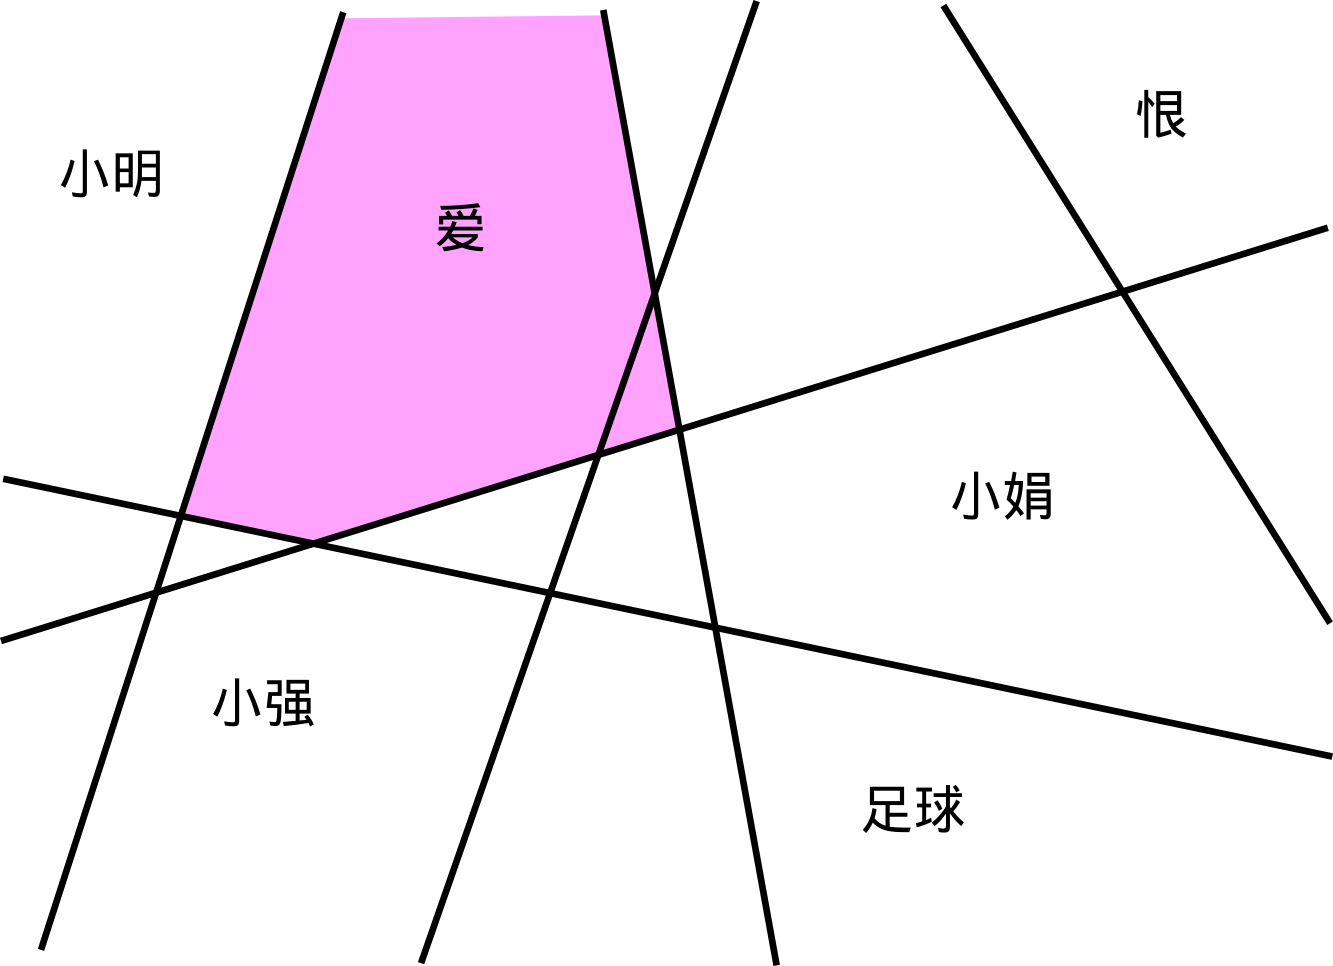
\includegraphics[scale=0.5]{distributive-vector-representation-linear.png}
\end{figure}

一粒神经元的公式是:  $y = \sigmoid (w^T x \leq b) $

(但如果只有一层神经元)那非线性函数可以不理(它不影响 decision boundary)。

$ (w^T x \leq b) $ 表示一个 hyperplane 的切割。

一个概念就是一组 hyperplanes 切割而成的多面体 (polyhedron),\\
\tab \tab $c : (Wx \leq B) $。\\
矩阵 $W$ 对应於一层神经网络中的 weights。

问题是这个表示法,如何表示乘积?  在这个表示法中,「线性无关」代表什么?

\subsection{「连续性」}

第二个问题是「连续」指的是什么。 例如命题 $P_1$ =「小明爱小娟」,$P_2$ =「小强爱踢足球」,那么由 $P_1$ 变化到 $P_2$ 必然会有 discrete jump,那是无可置疑的。 除非我们重新定义命题是像 $k_1 P_1+ k_2 P_2$ 那样的东西,才可以有「连续变化」;  这一点需要再加以精确化。

我发觉「连续空间」不是一个严谨的术语,因为在 discrete 空间中也可以定义 "continuous" 这概念,例如在 computer science 的 functional programming 里有 domain theory、 denotational semantics 等,常常谈到离散空间中的连续函数。 而且「可微分」的概念也有一些 generalizations,例如 Fr\'{e}chet derivatives(在泛函空间中)。

\subsection{近似}

那些算子或许可以合写成一个:
$$ T_1 v + T_2 v + ... + T_n v = \mathcal{T} v $$
然后合写后用 function approximation 来近似。

但这种近似必须有代价,否则违反了两项原则:
\begin{enumerate}
\item Turing 已经很有远见地意识到,逻辑推导的普适算法是不存在的,因为它违反了停机原理 (halting problem)。 后者是用 Cantor 的集合论中的 diagonal argument 证明的。 如果我们的优化算法必然会给出答案,而答案又可以转换回逻辑,那是不可能的。 所以在近似过程中必然会有某些误差。
\item 如果 $P \neq NP$,我们的算法也不可能总是在 polynomial time 之内回覆正确答案。
\end{enumerate}

还有一个 "second-order" 的想法。  在 first-order 我们的算子是这个形式:
$$ T: V \rightarrow V $$  
但 second-order 的做法是将所有\textbf{物体}都看成是算子,算子可以作用在算子之上,这似乎是一种 duality。 暂时还未知道细节。

如果我们简单地将 $\mathcal{T}$ 近似,那些逻辑推导就会有错误。  或者应用某个 duality 之后,近似的做法会有较好结果?

\subsection{逻辑是什么?}

总结一下逻辑是什么:  一个逻辑系统 $\mathcal{L} = \{ C, P, d(\cdot,\cdot), \supseteq \}$:
\begin{enumerate}
\item 原子概念集 $C \ni c_1, c_2, ...$
\item 命题集 $P \ni p_1, p_2, ...$ (可以限制在简单关系 $a\, R\, b$)
\item 连结词 (conjunction) $p_1 \wedge p_2$ 或 $p_1 + p_2$
\item 概念之间的距离 $d(c_1, c_2)$
\item 概念之间的偏序 (partial order) $c_1 \supseteq c_2$
\end{enumerate}
我们想把这个结构映射到 Banach 空间。 那个 $\supseteq$ 关系可能要用空间中的 cones 来表示,而且用 hyperbolic geometry 可能比较好;  这是后话。

\section{Neural Tensor Network}

Andrew Ng 是香港人,Coursera 的 machine learning 教授,他在 Stanford,最近加入了百度。 他和合作者提出了 NTN 模型\cite{Socher2013}:
$$ \top(a\, R\, b) = u^T \; \sigmoid \, (a^T \, U \, b + W {{a}\choose{b}} + c ) $$
$\top(a\, R\, b)$ 表示 $a\, R\, b$ 这个关系的\textbf{强度}。\\
$U$ 是一个 tensor,取两个向量 $a, b$ 给出第三个向量 $a^T \, U \, b$(它服从张量的双线性性质)。\\
$W$ 是一个矩阵,$W {{a}\choose{b}}$ 是一层传统的神经网络,$\sigmoid$ 是一个非线性函数。\\
$u^T$ 是一粒神经元,作用是把各个分量加起来,得出一个数。

\section{Paul Smolensky's tensor representation}

Paul Smolensky 的书是《The harmonic mind》(2006)\cite{Smolensky2006},第一卷是 AI 理论,第二卷是语言学理论。

他提出用张量来表示关系:
\begin{eqnarray}
father(john, pete) & \Leftrightarrow & father \otimes john \otimes pete \nonumber \\
Var_1 : val_1, Var_2 : val_2 & \Leftrightarrow & Var_1 \otimes val_1 + Var_2 \otimes val_2 \nonumber 
\end{eqnarray}
第二句的意思是,variable 1 的值是 value 1,variable 2 的值是 value 2。 

我在博客\footnote{\href{http://geniferology.blogspot.hk/2015/03/what-are-tensors.html}{blog post}}上解释过,tensor 是所有 bi-linear forms 的 universal form。 如果有向量空间 $U$ 和 $V$,
\begin{eqnarray}
T: & U \otimes V \rightarrow W \nonumber \\
t: & u \otimes v \mapsto w \nonumber 
\end{eqnarray}
那么在 $U, V$ 中线性无关的 $\{u_1, ..., u_m \}$ 和 $\{ v_1, ..., v_n \}$,它们的乘积 $\{ u_i \otimes v_i \}$ 在 $W$ 中仍然是线性无关的。  换句话说:
$$ \mbox{线性无关集} \otimes \mbox{线性无关集} \mapsto \mbox{线性无关集} $$
而这正是我们需要的,因为根据「scalar = 逻辑命题真假值」的诠释,这正是命题之间不「相撞」的条件。

Antony Browne \& Ron Sun 的较早的论文《Connectionist inference models, 2001》\cite{Browne2001}有讲述更多 neural-symbolic integration 的做法。

\section{Metric embedding}

最近有一本新书:[Mikhail Ostrovskii 2013] \textit{Metric embeddings: bi-Lipschitz and coarse embeddings into Banach spaces}\cite{Ostrovskii2013},它似乎正正讲述了我们将 logic 嵌入到「连续空间」的问题。

What is the bi-Lipschitz condition?  A map $f: X \rightarrow Y$ is called a \textit{C-bi-Lipschitz embedding} if there exists $r > 0$ such that
$$ \forall u,v \in X, \;\; r\, d_X(u,v) \leq d_Y(f(u), f(v)) \leq r C\, d_X(u,v) $$
for some $C < \infty$.  The smallest constant $C$ for which there exists $r > 0$ such that the above is satisfied is called the \textit{distortion} of the map $f$.  这似乎定义了「远的保持远、近的保持近」的意思。

\section{SVMs and the kernel trick}

印象中 \textbf{SVM} (support vector machine) 似乎可以将非凸的问题转化成凸优化的问题; 可不可以将这个想法应用到我们的问题上呢?

SVM 的算法,首先用 kernel trick 将 data points 转换到高维空间,然后在高维空间中进行线性的 hyperplane 分割。

所谓 \textbf{kernel trick} 是指: 给定一个 inner product,它暗含了一个到高维空间的转换 $\phi$ (但这个转换不需要真的计出来)。

%A given dot product implicitly defines a transformation $\phi$ into higher dimensional space.  In such a space the data set might be linearly separable.

\begin{figure}[H]
\centering
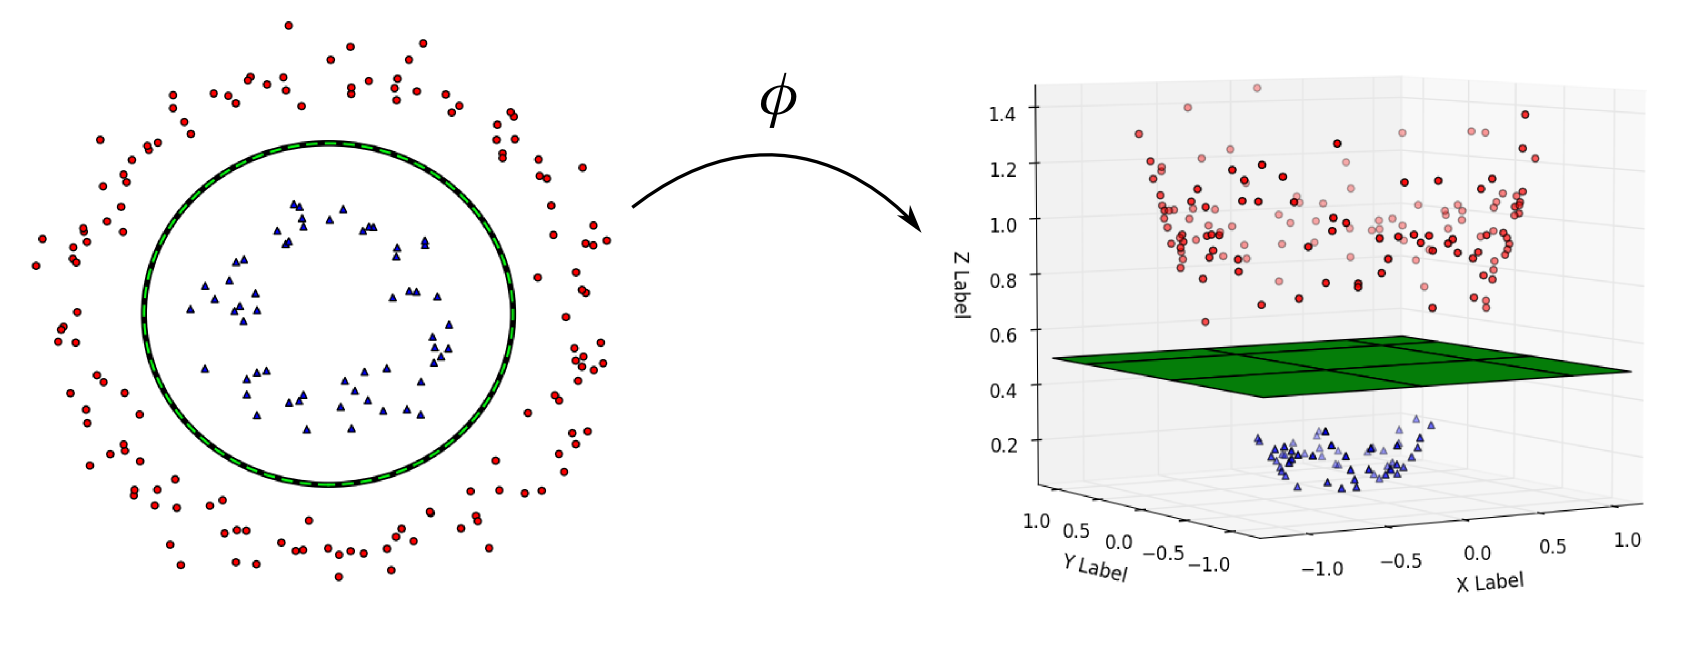
\includegraphics[scale=0.6]{kernel-trick.png}
\end{figure}

而,在高维空间中用线性分割,那 error term 是一些正交距离,所以是 \textbf{quadratic form},所以这问题是\textbf{凸优化}。

%The \textbf{quadratic form} comes from the linear separation, and that's why the problem is a convex optimization problem.

我们的问题是性质不同的,但两者似乎有些相似... 

\begin{comment}

读者可能好奇我搞的 Genifer 4 是什么,其实没有很大不了,基本上是想将逻辑转移到\textbf{连续空间},再应用连续逼近的技巧,例如梯度下降法 (gradient descent)。

最近一年时间,费了九牛二虎之力,才将逻辑变连续了(甚至这一步也未完善),但至少可以将 inductive learning 的问题变成数学上的 continuous optimization 问题。

然后才发觉,最快的 optimization 算法,是基於 convex (凸性)的技术。  如下图的 fitness landscape,一个是凸的,另一个是不规则的:\footnote{from Charles H Martin's \href{https://charlesmartin14.wordpress.com/2013/11/14/metric-learning-some-quantum-statistical-mechanics/}{blog}.}
\begin{figure}[H]
\centering
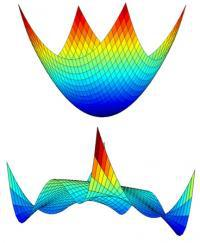
\includegraphics[scale=0.6]{convex-and-nonconvex.jpg}
% \caption{Convex and non-convex fitness landscapes.}
\end{figure}

而如果没有了凸性,便要用到 genetic algorithms、branch-and-bound 之类的技巧。 那些技巧我在 computer science 一早知道了,而且毋须用到连续性和梯度,令我失落地感到「多此一举」  \sadface

后者虽然也可以很快,但它们属於 heuristics (窍门),也就是没有速度的保证。  由於机器学习的复杂性极高,在没有保证下 我们敢不敢尝试用那些 heuristics 呢?  比方说,你愿不愿意投资几百万的赌注在 Genifer 3.0 上?

数学的确很神奇,它不断在进步,可惜进步得很缓慢。 现时的一个前沿是将 convex 推广,但我暂时还未听过有什么突破(但我只是初学者,还未堪察过这範围的文献)。 如果有的话,那将会是 ground-breaking,但这不是普通人能做到的,甚至大部分数学家也不能。

暂时可以做的大概是:
\begin{itemize}
\item 找一个 non-convex 但仍然可以快速解决的问题,然后将我们的问题转化成那问题。
\item 改变原问题的 representation,这需要很有创意。 甚或将 optimization 问题改变成 solve equation 的问题、等。
\item 然后试试那 fitness landscape 会不会有好一点的性质;  需要实验,把那些 error surface 描出来。
\item 放弃 convex,仍然可以用其他 global optimization 的方法,如: 遗传算法、branch-and-bound、convex-concave / DC programming、神经网络的 back-propagation、simulated annealing 等。 但如上所述,有些技巧已经不需连续性,可以回到 Genifer 3。
\end{itemize}

馀下的篇幅,谈谈我关於逻辑连续化的尝试,日后可能还会有用(但也可能是 dead-end)。

\section{逻辑的连续化}

基本上我是想建立这个对应 (correspondence):
\begin{center}
\colorbox{yellow}{\parbox{0.75\textwidth}{
\begin{tabular}{ccc}
KB (knowledge base) & $\Leftrightarrow$ & 连续空间 \\
逻辑 rules & $\Leftrightarrow$ & 连续空间上的非线性算子\\
学习逻辑 rules & $\Leftrightarrow$ & 在泛函空间中寻找算子\\ 
\end{tabular}
}}
\end{center}

即使连续化之后还有 non-convex 的问题,暂且不提。 单是连续化已经很难,因为传统逻辑的结构很复杂。

很多逻辑理论,用的是数学符号表述,但其实和数学的其他分支没有什么联系,只是一堆符号而已。 如果要真正有用,必须从逻辑「搭桥」(bridge) 到其他数学分支上。 我发觉最容易是通过(抽象)代数,因为有了代数表达式之后,可以较易看到和其他数学的关系。

\section{逻辑是什么?}

逻辑分为 \concept{propositional logic} 和 \concept{predicate logic},前者 isomorphic to Boolean algebra 所以比较易懂,数学上也较简单; 后者是很难用代数描述的,例如要用到 Tarski 所创的 cylindric algebra,在逻辑圈子以外很少人懂,而我正试图用另一个办法,其想法是基於组合逻辑 (combinatory logic) 和关系代数 (relation algebra)。 \footnote{所谓组合逻辑的意思是: 将谓词逻辑的 $R(a, b)$ 写作代数式的 $R \,a\, b$ 或 $a \,R\, b$,例如 $loves(john, mary)$ 变成 $john \cdot loves \cdot mary$。 关系代数是组合逻辑的一个特殊形式。}

% 很多数学专业的人没有时间钻研 predicate logic,所以我很寂寞,但我希望你们能暂时忽略一些 details,而我们可以尽量讨论一些具体的数学问题。

首先很明显的是,逻辑 formulas 可以表达成树状结构,而树状结构也可以很容易表示为 sum-product 的代数结构,例如(甚至是二元树):
\begin{figure}[H]
\centering
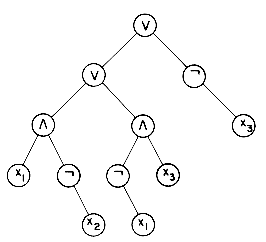
\includegraphics[scale=0.5]{logic-formula-tree.jpg}
% \caption{Convex and non-convex fitness landscapes.}
\end{figure}

但在向量空间中表示会有问题,因为向量有加法,但乘法没有明显的候选人。 例如,如果\formula{小明$\cdot$爱$\cdot$小娟} 和 \formula{小强$\cdot$爱$\cdot$踢$\cdot$足球} 这两句不相关的句子在\concept{概念空间}上的位置「相撞」或者不合理地接近,会是很不妥的。 

\section{Cayley graph}

较早时我试过的一个做法是用 Cayley graph,但后来发觉不好用。

Cayley graph 的原理很简单,例如下图是 $\{ a, b \}$ 两个元素产生的自由群 (free group),乘积用线连起来:
\begin{figure}[H]
\centering
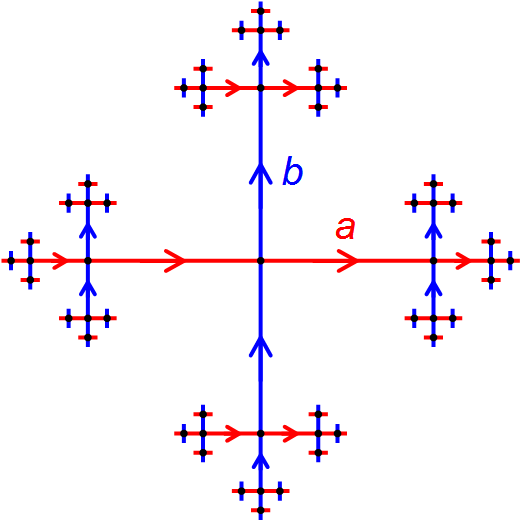
\includegraphics[scale=0.25]{cayley-graph.jpg}
\end{figure}

在人工智能中还有\concept{本体论} (ontology) 这个概念,例如\, \formula{猫 $\subseteq$ 动物}。 本体可以表达成一个阶级分类 (hierarchical cluster),这又可以变成圆形或球形:
\begin{figure}[H]
\centering
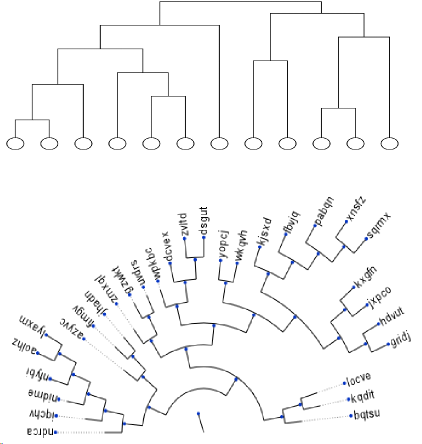
\includegraphics[scale=0.5]{ontology-ball.png}
\end{figure}

我企图将本体论和 Cayley graph 的想法结合起来: Cayley graph 中每个 node 是一个\concept{概念}(例如 \formula{爱} 或 \formula{足球}),而每个概念也可以在球状的本体中找到位置。 问题是本体球本身已经有 hierachical 结构,我想把球状本体「嵌入」到 Cayley graph 的節點中,似乎不易。

再者,当 Cayley graph 的分支数目增大时,看起来越来越「不自然」; 例如这只是 $n=5$ 的情况:
\begin{figure}[H]
\centering
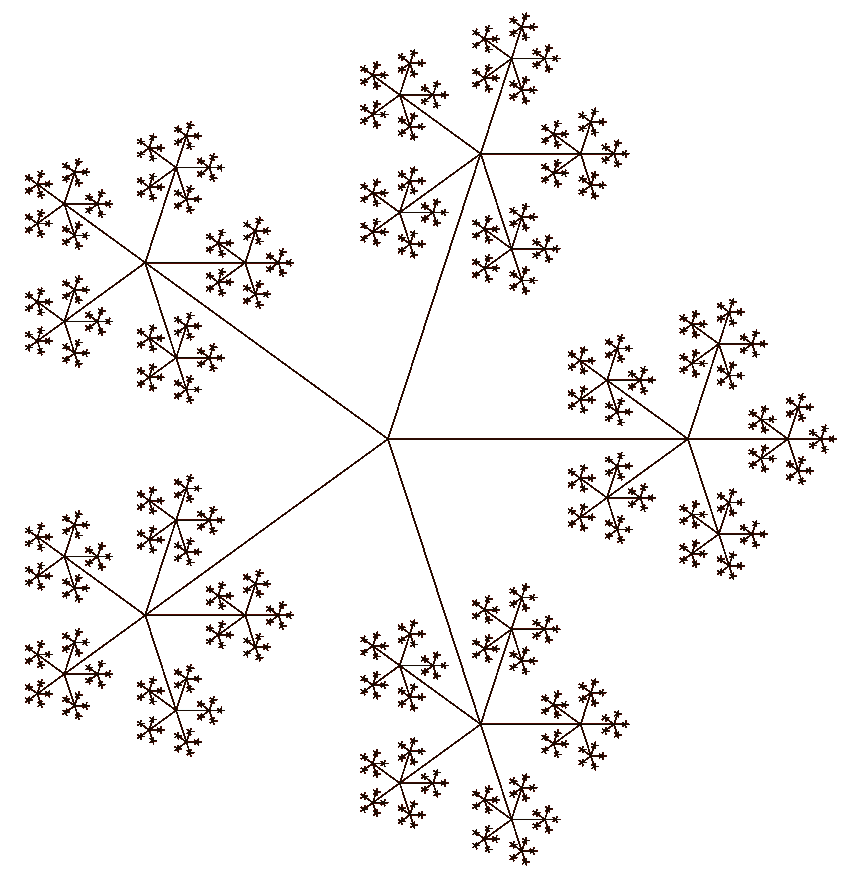
\includegraphics[scale=0.25]{cayley-graph-5.png}
\end{figure}
原因是,Cayley graph 其实是一个 fractal structure! 我原希望得到「连续」的效果,但在 Cayley graph 上从一个节点跳到另一个节点是\textbf{不连续}的。

虽则如此,Cayley graph 还有一个好处,就是它可以嵌入到 hyperbolic disc 上,这个圆盘有\textbf{双曲几何} (hyperbolic geometry) 的尺度(这在 M C Escher 设计的艺术中常见到,即圆盘越接近边缘的空间尺度越缩小):
\begin{figure}[H]
\centering
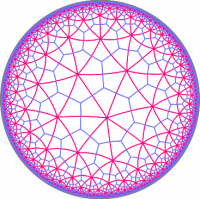
\includegraphics[scale=0.75]{hyperbolic-disc-beautiful.png}
\end{figure}

在双曲几何中直线变成圆弧,而神经网络将空间切割的方法也包含线性的 $Y = \sigmoid(\sum W_i X_i)$,或许可以制造一种 hyperbolic neuron?  可惜因为不连续的问题,这方案暂时搁置。

\section{Distributive vector representation (DVR)}

这是一个较好的方案,似乎可以解决\textbf{连续性}的问题。

在 DVR 架构下,知识是用一个很长的 vector 表示:
$$ K = \mathbf{v} = (v_1, v_2, ... , v_n) $$
这在神经网络中很常见。  意思是: 每个\textbf{概念}不是用单一的神经元 (即一个 $v_i$) 表达,而是用整个 layer 的神经元表达 (即 $\mathbf{v}$)。 在这种表述下,一个概念是空间中的一个或多个 regions,它们可以是 disjoint 的。

例如,向量空间的维数 $n=2$ 时,可以有这样的例子:
\begin{figure}[H]
\centering
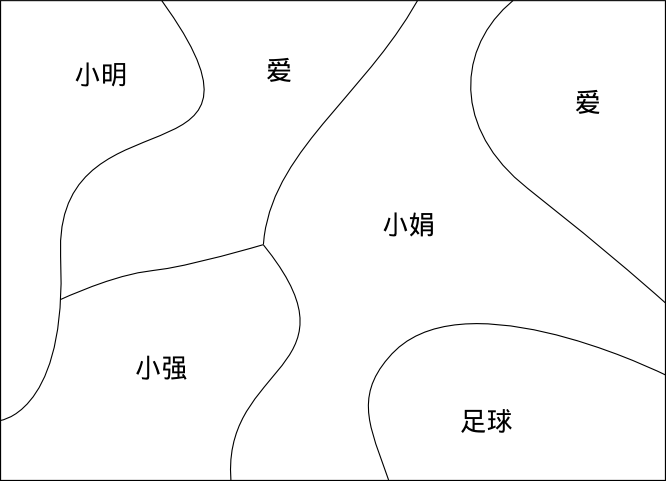
\includegraphics[scale=0.5]{distributive-vector-representation.png}
\end{figure}

向量可以\textbf{相加},相加的意思是\concept{叠加} (superimpose),这概念也来自神经网络。 例如 \formula{小明$\cdot$爱$\cdot$小娟} 和 \formula{小强$\cdot$爱$\cdot$踢$\cdot$足球} 这两个 formulas 可以同时叠加在 $K$ 上,表示这两句句子同时是真的。 在概念之间互不「相撞」的情况下,这是可行的。

但仍有一个问题: 当命题重复时,命题的真值不会变双倍(例如重复说「小明爱小娟」两次),换句话说,$a \wedge a = a$,但向量的加法会变双倍,除非我们选另一个\textbf{域}上的向量空间 (vector space over a field),在这个域里 $ 1 + 1 = 1 $ 或什么。 这也是一个未解决的细节。

暂时也不理\textbf{乘法}的问题,第7节我们再讨论怎样表示乘积。

\section{逻辑推导}

逻辑的基本运算,是由一个 KB (\concept{knowledge base}) 推导出新的逻辑句子,即  deduction。 ``KB'' 这术语来自经典 AI,在新表述下简称作 $K$。

Deduction 的基本动作是 apply rules to facts。 Deduction 可以用算子 $T$ 表示:
$$ T: K \mapsto K .$$
但 $T$ 是\textbf{非线性}的。

$T$ 对应於一个 logical rule。  例如一个经典例子是「爷爷」的定义:\\
\tab \formula{ 爷爷(X,Z) $\leftarrow$ 爸爸(X,Y) $\wedge$ 爸爸(Y,Z)}

这个 deduction 动作,首先要做 pattern matching ,然后才能 apply。

所以有这样的对应:
\begin{center}
\colorbox{yellow}{\parbox{0.55\textwidth}{
\begin{tabular}{ccc}
deduction & $\Leftrightarrow$ & apply operators \\
pattern matching & $\Leftrightarrow$ & filter: $K \rightarrow K$ \\ 
\end{tabular}
}}
\end{center}

举例说,我们已知这些事实:\\
\tab \formula{爸爸(小明, 小强)} \\
\tab \formula{爸爸(小强, 大强)} \\
而我们必须找到 {小明/X, 小强/Y, 大强/Z} 这个 substitution,才可以 apply 上面那 rule。  找这个 substitution 的操作叫 pattern matching,经典的\textbf{归一化}算法 (unification algorithm) 可以做到。

这就是 $T$ \textbf{非线性}的原因。  因为对於不同的 $K$,$T$ 的作用通常是 0,除非 pattern matching 成功,$T$ 的作用才是非零。 (当然,实际上我们会将 $T$ 变 smooth,所以上面的「= 0」应该说是「接近0」。)

在一个 AI 系统里有很多 rules,对应於 $T_1, T_2, ...., T_n$。  分别将 $T_i$ 作用在 KB 上,然后再叠加在一起,这就进行了推导的一步 (single step)。  但由於 $T_i$ 是非线性的,求和与 $T_i$ 不可交换 (commute)。

单步的推导是:
     $$ K' = \sum T_i (K) $$
而 KB 的所有逻辑结论 (full logical consequence) 就是:
\begin{eqnarray} \nonumber
K^\infty & = & \mbox{以上的单步重复无限次} \\ \nonumber
         & = &  (\sum T_i) ^\infty (K^0) .
\end{eqnarray}

\section{学习}

学习算法是人工智能的瓶颈,有了好的 inductive learner,其他细节只是细节(例如用 reinforcement learning 解决)。

逻辑的 inductive learning 有一个\textbf{双重结构}的特点,就是学习需要用到推导,但推导本身也是是一个复杂算法。

换句话说,先用推导得到 $K^\infty$ (这本身需要算子的 iteration):
$$ K^\infty = (\sum T_i) ^\infty (K^0) .$$
然后将结果 $K^\infty$ 和理想的 $K^*$ 比较,得到误差,而我们目标是找出一套 $T_i$ 令这误差最少。 $T_i$ 活在非线性算子的空间中。

逻辑上我们希望达到的是:
$$ K^0 \cup \{ T_i \} \models E $$
其中 E 是新的需要解释的例子或经验 (experience)。 理想的答案是 $K^* = K^0 \cup E$。 

误差 $\mathcal{E}$ 是推导出来的 $K^\infty$ 减去理想的 $K^*$:
$$ \mathcal{E} = K^\infty - K^* = (\sum T_i) ^\infty K^0 - (K^0 + E) . $$

如果 $T_i$ 是可微的,梯度 $\partial\mathcal{E}/\partial T_i$ 存在,我们就可以用梯度下降法。

和一般常见的的优化算法比较,例如 Newton-Raphson 只是一个算子的 iteration,
$$ x^\infty = T^\infty x^0 $$
就是所需答案。

和传统神经网络的 back-propagation 比较,back-prop 的算法是:\\
\tab (一粒神经元) \tab $y_j = \sigmoid( \sum W_{ij} x_i )$ \\
\tab (多层结构) \tab $\mbox{output} = y_0 \circ y_1 \circ ... \circ y_n (\mbox{input})$ \\
\tab (update 法则) \tab $ \mathbf{W}' = \mathbf{W} + \alpha \; \partial \mathcal{E} / \partial \mathbf{W} $

两者比较:
\begin{itemize}
\item back-prop 的算子 $ y_0 \circ y_1 \circ ... \circ y_n $ 是来自很多层的神经网络结构,所以 back-prop 可以看成是 error 在\textbf{空间}中的传播。
\item 我们的 iteration 是在时间中发生的,但似乎没有本质上分别。
\end{itemize}

我现时认为问题是: 那 $K$ 的空间可能太大(即使维数不大),因为它包含所有逻辑式子,而且,如果没有任何 approximation 的话,这问题完全和逻辑学习的原问题一模一样,这新的做法不会有任何改进,那顶多是原问题在连续空间中的 relaxation。 应该利用连续空间的 function approximation 来做点\textbf{一般化} (generalization)。

但逻辑中也有它的一般化结构。  一般化的目的是\textbf{压缩},也可以说学习就是压缩。  逻辑学习本身就是一种复杂度很高的压缩法(所以它才那么慢),那 $A \subseteq B$ 的 subsumption 关系,造成一个阶层 (hierarchical) 分类结构,这分类法相当於把数据的复杂性取对数 (take the logarithm of the size of the knoweldge base),就像二分搜索 (binary search) 那样。  但因为逻辑学习有双重的 exponential 复杂度,可能单使用这个技巧还未够?

研究逻辑学习的 Stephen Muggleton 在 2002 年关於用\textbf{遗传算法}做逻辑学习说:
\begin{quote}
\textit{「在一阶逻辑学习系统里,验证假设的方法通常是呼叫一个逻辑证明器(例如 Prolog 解译器)去找出那假设对学习例子的正和负覆盖。  已知道这是一阶概念学习中复杂而费时的一步。 在基因学习里,这情况更差,因为每一代都有一群假设要验证。」}\footnote{\, \textit{"The usual way for evaluating a hypothesis in first-order concept learning systems is to repeatedly call a theorem prover (eg Prolog interpreter) on training examples to find out positive and negative coverage of the hypothesis.  This step is known to be a complex and time-consuming task in first-order concept learning.  In the case of genetic-based systems this situation is even worse, because we need to evaluate a population of hypothesis in each generation.  This problem is another important difficulty when applying GAs in first-order concept learning."}}
\end{quote}

压缩的方法必须是 ``semantic distance preserving'',意即: 在语义空间中相似的点被压缩到相邻的逻辑範式。

问题似乎是: 法则的诱导似乎不能单是基於语法。 概念阶层的诱导是基於: Liebniz 和 $a\, R\, b$。

Liebniz extensionality:
\begin{eqnarray}
xZ \rightarrow yZ \Leftrightarrow x \supset y \\
Zx \rightarrow Zy \Leftrightarrow x \supset y
\end{eqnarray}

The relation of subsumption is \textit{intrinsic} to the logic.  

\section{乘法}

暂时还不清楚怎样表达乘法,例如 \formula{小明$\cdot$爱$\cdot$小娟} 这样的乘积。 

其中一个方案由 Geoffrey Hinton 提出: 每个概念是一个\concept{矩阵} (matrix),如果概念 $a$ 和 $b$ 有关系 $a\, R\, b$,则代表它们的矩阵会服从 $ AR = B $,而这些矩阵在矩阵空间中的位置是要学习得来的。  但这方法似乎比较麻烦,因为要判断哪个元素跟著哪个元素,要靠矩阵乘法得出来。

第二个方案是使用\concept{张量积} (tensor product),但张量积的 dimension 很大,而且随著乘积的长度增加。 Paul Smolensky 的书《The harmonic mind》(2006) 第一卷有描述他发明的 distributive tensor product representation,我迟些有空再解释它。 

第三个方案,出自《Quantum physics and linguistics》(2013) 这本论文集。 他们使用的是\concept{幺半範畴} (monoidal categories),那是一种又有乘积又可以组合 (compose) 的範畴。 它的定义包括:
\begin{itemize}
\item objects: $X, Y, ...$
\item morphisms: $f: X \rightarrow Y$
\item composition: $f \circ g : X \rightarrow Z$
\item grouping objects into: $X \otimes Y$
\item a special object for the ``empty system'': $I$
\item parallel composition: for $f_1: X_1 \rightarrow Y_1$ and $f_2: X_2 \rightarrow Y_2$ \\
\tab \tab $f_1 \otimes f_2: X_1 \otimes X_2 \rightarrow Y_1 \otimes Y_2$
\end{itemize}
它的代数运算可以用一些\concept{扭} (braid) 图像地表示:
\begin{figure}[H]
\centering
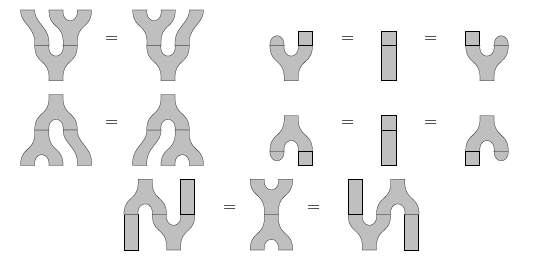
\includegraphics[scale=0.75]{frobenius_algebra.jpg}
\end{figure}
这似乎是是一个很 general 的结构(包含 tensor product?)  这本书其中一个主旨就是说这个範畴能够涵盖所有自然语言的语法。 但我暂时未有空研究它。

另一个方案是我创的,想法是: 可以把下面这样的一个时间函数看成一个连续的时间\textbf{序列}:
\begin{figure}[H]
\centering
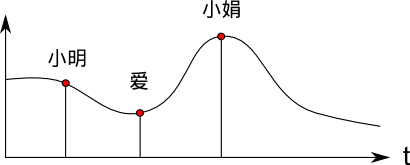
\includegraphics[scale=0.75]{continuous-time-sequence.png}
\end{figure}
而乘积也是一个 discrete 序列,可以把它连续化变成时间 t 的\textbf{连续曲线}。

这些曲线在 $K \times t$ 的空间中是像这样的:
\begin{figure}[H]
\centering
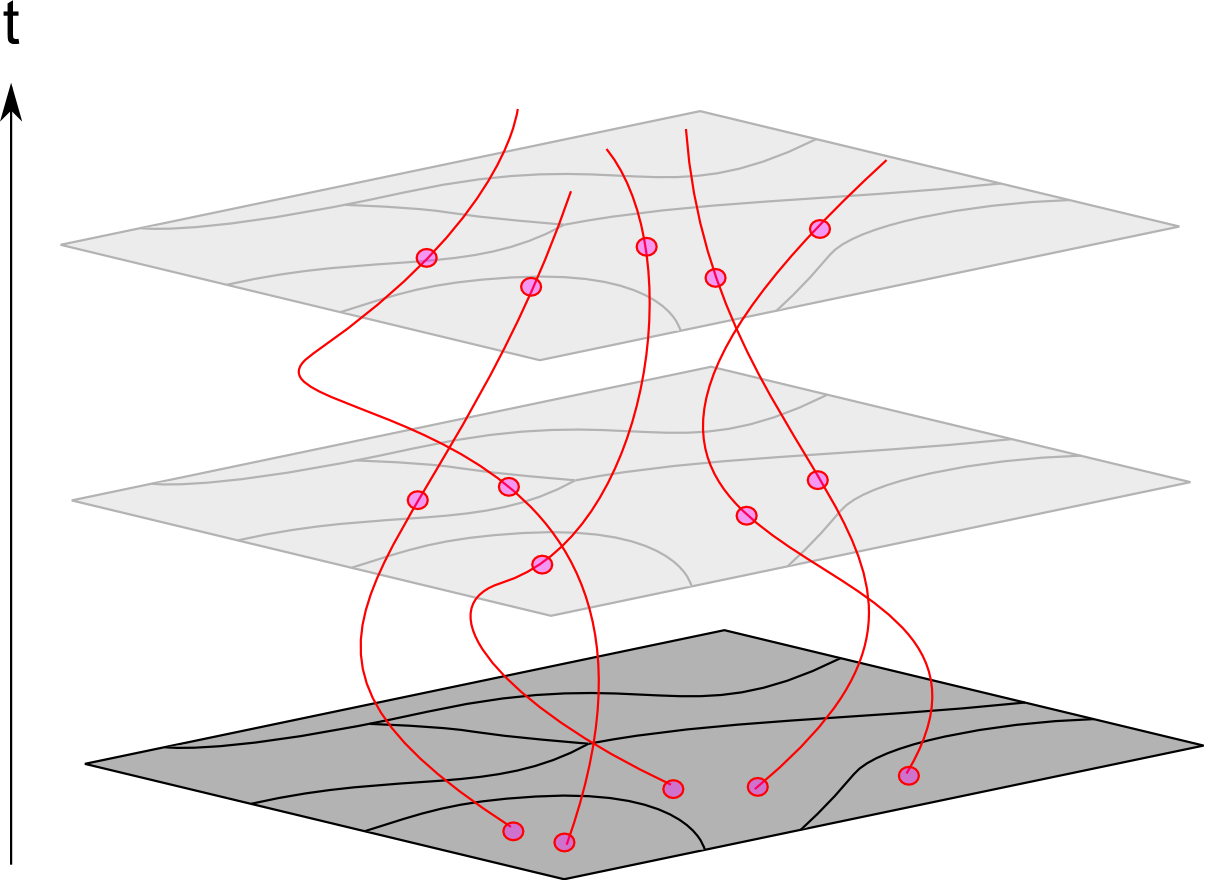
\includegraphics[scale=0.75]{polynomial-hairs.png}
\end{figure}

这些曲线可以用 spline 表示,也就是\concept{多项式} (polynomial)。  这样或许可以用到 algebraic geometry (现代数学里很深奥的一个分支)里面的技巧。  一个多项式可以用它的 coefficients 表示,那就是一串数,很方便。 而多项式之间的变换也可以用多项式来描述,形成\concept{对偶空间} (dual space),这类似於 logic 中,rule 可以作用在其他 rules 之上。 

\section{Formal power series}

幂级数的形式是这样的:
$$ \sum k_i a^i $$
但如果 $a_i$ 不是普通的数,我们不能用普通加法求和,所以叫它做\concept{形式级数} (formal series)。

抽象地说,设 $A$ 是一个\textbf{原子概念}的集合,例如 $\{ \mbox{爱}, \mbox{恨}, \mbox{男人}, \mbox{女人}, ... \}$ ,$A^*$ 就是这些概念可以组成的所有句子。 给这些句子乘上一些系数再加起来,例如:\\
\tab 0.8 \formula{小明$\cdot$爱$\cdot$小娟} + \\
\tab 0.3 \formula{小娟$\cdot$爱$\cdot$小明} + \\
\tab 0.9 \formula{小娟$\cdot$爱$\cdot$小强} + \\
\tab ... \\
系数 $k_i \in K$ 而 $K$ 可以是任何\concept{半环} (semi-ring),我们可以把 $K$ 看成是\textbf{逻辑真假值}的半环。 

所有如上的形式级数,记作 $K\llangle A\rrangle$。

形式级数和\concept{有限自动机} (finite state machine, FSM) 有密切关系: FSM 可以用来辨认\textbf{形式语言} (formal languages)。 一个形式语言 $L$ 可以是任何 $A^*$ 的子集。  如果 $L$ 包含某句句子,则给这句子系数 1,否则系数 0。  於是我们得到一个代表那形式语言的形式级数。

并不是任何形式语言都可以被 FSM 辨认。

如果可辨认,则对於这语言内的每个字母 (``原子概念''),可以建立一个 $M_{n \times n}$ 矩阵,其 $M_{pq}$ 元素视乎自动机由状态 $p$ 到 $q$ 有没有 transition(如果有是 1,没有是 0)。

这些矩阵的乘法满足概念的 monoid 乘法,例如 : $a \cdot b \cdot c \,\times\, d \cdot e \cdot f = a \cdot b \cdot c \cdot d \cdot e \cdot f$。

在\concept{表示论} (representation theory) 里,我们说这些矩阵是这个 monoid 的 matrix representation。

根据表示论,一个环 $K$ 乘上一个 monoid $A$ 会得到一个 $K$-module,所以 $K \llangle A \rrangle$ 可以看作是一个(左边的) $K$-module。

Module 的存在代表 representation 的存在。 (著名的犹太裔女数学家 Emmy Noether 开创用 module 研究 representations 的做法。)

而刚才也看到, FSM 可辨认 $\Rightarrow$ 可以建立 matrix representation。

所以,「FSM 可辨认」的另一个定义就是「存在 matrix representation」,这又可以再定义为「有某种 finitely generated $K$-submodule,它包含 $S \in K \llangle A \rrangle$」($S$ 是那个语言的形式级数)。

以上的内容部份摘自 Encyclopedia of mathematics《Noncommutative rational series with applications》(2011 剑桥大学出版)。 

\begin{center}
\colorbox{yellow}{\parbox{0.9\textwidth}{
\begin{tabular}{ccc}
% ??? logic formulas & $\Leftrightarrow$ & algebra over the ring of truth values \\
facts (propositions) & $\Leftrightarrow$ & monoid words \\
KB & $\Leftrightarrow$ & formal series \\
rules & $\Leftrightarrow$ & non-linear operators acting on formal series \\
\end{tabular}
}}
\end{center}

\section{储存器}

最后还不得不提,经典逻辑的结构实在太复杂了,我们的烦恼还未完...

在 Genifer 3 white paper 里,我解释过需要引入有「储存器记忆」的逻辑。  那就是说需要加进一些逻辑「动作」,容许储存器的读和写。

\begin{center}
\colorbox{yellow}{\parbox{0.85\textwidth}{
\begin{tabular}{ccc}
memory register & $\Leftrightarrow$ & vector space $K \times t$ \\ 
actions & $\Leftrightarrow$ & some meta-operations (?) over registers\\
\end{tabular}
}}
\end{center}

实在太麻烦了,今次到此为止,下次再 update 吧!

\section{徵求合作者}

例如,我去过 香港科技大學 找人,但那研究生说他们簽了合约,规定不准幫外面工作(大概这是大学控制知识产权的一种措施)。

\begin{tabular}{|c|c|c|c|}
\hline
\textbf{Notation} & \textbf{Meaning} & \textbf{Example } \\
\hline
$A \supset B$ & concept A is a superset of concept B &
$animals \supset cats$ \\
& &  \english{cats are animals} \\
\hline
$A \ni B$        & concept A contains an element concept B &
$a \circ bird \supset tweety$ \\
& & \english{Tweety is a bird} \\
\hline
$A \rightarrow B$ & proposition A entails proposition B &
$bird \, X \supset can \, fly \, X$ \\
& & \english{If X is a bird X can fly} \\
\hline
\end{tabular}

\begin{figure}
\centering
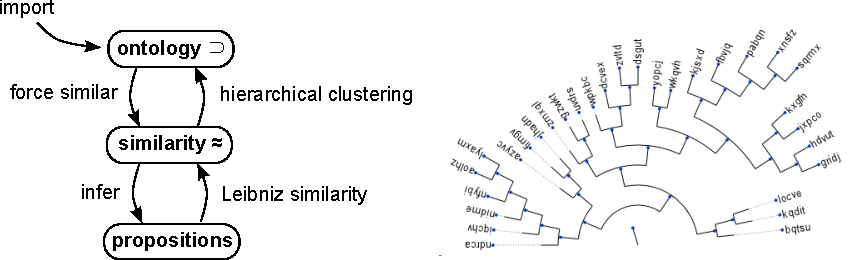
\includegraphics[scale=0.8]{ontology-relations-relations.pdf}
\caption{Left: relations between ontological data.  Right: a random example of dendrogram.}
\label{fig:ontology-relations-relations}
\end{figure}

\section*{Appendix: XXXX}

\section*{Acknowledgments}

I am heavily indebted to Pei Wang \cite{Wang2006} \cite{Wang2013} and Ben Goertzel \cite{Goertzel2011} for their seminal contributions to AGI.  To Abram Demski and Russell Wallace -- we have spent years exploring many ideas in logic.  Also thanks to Matt Mahoney, Jeff Thompson for discussions of the draft.  William Taysom, Seh, and Joseph Cheung helped implement the code.
\end{comment}

\bibliographystyle{plain} % or number or aaai ...
\bibliography{AGI-book}

\onecolumn

% Bigger figures

\end{document}
